\documentclass[11pt,a4paper]{article}

% ---------- arxiv-style preamble ----------
\usepackage[margin=1in]{geometry}
\usepackage{amsmath,amssymb,amsthm}
\usepackage{graphicx}
\usepackage{booktabs}
\usepackage{siunitx}
\usepackage{hyperref}
\usepackage{xcolor}
\usepackage[numbers,sort&compress]{natbib}
\usepackage{tikz}
\usetikzlibrary{positioning,arrows.meta}
\usepackage{pgfplots}
\pgfplotsset{compat=1.18}
\usepackage{caption}
\usepackage{listings}
\usepackage{array}
\captionsetup{font=small,labelfont=bf}
\hypersetup{
  colorlinks=true,
  linkcolor=blue!50!black,
  citecolor=blue!50!black,
  urlcolor=blue!50!black
}

% ---------- emoji tier badges ----------
% text colour badges (font-independent — no emoji glyph dependency)
\newcommand{\tierbadge}[2]{\textcolor{#1}{\textbf{[#2]}}}
\providecommand{\tierBlue}{\tierbadge{blue!60!black}{BLUE}}
\providecommand{\tierGreen}{\tierbadge{green!45!black}{GREEN}}
\providecommand{\tierYellow}{\tierbadge{yellow!50!black}{CITE}}
\providecommand{\tierOrange}{\tierbadge{orange!80!black}{ORANGE}}
\providecommand{\tierRed}{\tierbadge{red!75!black}{RED}}

\title{
  \textbf{The in-silico design space for an androgenetic-alopecia\\
  complete-restoration cure collapses to a single measurable axis}\\[4pt]
  \large A negative result: every axis orthogonal to anagen efficacy ($E_{max}$)
  is deterministically settled, and three candidate mechanisms are falsified
}

\author{
  \texttt{demiurge} maintainers\\
  \normalsize\textit{dancinlab}\\[2pt]
  \normalsize\href{https://github.com/dancinlab/demiurge}{\texttt{github.com/dancinlab/demiurge}}
}

\date{\today}

\begin{document}

\maketitle

% =========================================================================
\begin{abstract}
Androgenetic alopecia (AGA) is partially reversible but has no disease-modifying
cure. We asked, purely in silico, whether a four-arm complete-restoration program
--- (1) reactivating dormant follicle stem cells, (2) reversing miniaturised
follicles, (3) permanently locking the corrected state, and (4) de-novo follicle
neogenesis in fibrosed regions --- can reach a pre-registered $\geq 90\%$
restoration-and-no-relapse cure gate, and which design variable controls that
gate. Across fourteen deterministic probes (DC1--DC14) we score each design axis
(mechanism choice, dosing sequence, lock timing, delivery cargo-fit, neogenesis
spacing) and propagate the single unmeasured efficacy parameter $E_{max}$. The
headline finding is negative and structural: once every in-silico axis is
resolved, the cure gate \emph{collapses} to a one-parameter condition --- it
closes iff $E_{max}\geq 0.96$ --- so every axis orthogonal to $E_{max}$ is ruled
out as the determinant. Crucially, $E_{max}$ is \emph{not} a from-scratch wet-lab
unknown: published minoxidil/finasteride dose-response data anchor the
current two-arm ceiling at $E_{max}\approx 0.59$--$0.80$ of normal productivity ---
a \emph{biological}, not pharmacological, plateau that coincides exactly with the
$25\%$ fully-fibrosed follicle fraction those drugs cannot reach. The cure gate
therefore reduces to a two-number \emph{in-vitro} target --- reactivation efficacy
$\eta_{\text{react}}{\to}0.95$ and neogenesis efficiency $\eta_{\text{neo}}{\to}0.84$
--- both bracketable on organoid platforms. We further show (DC14) that with
\emph{today's} human neogenesis efficiency ($\leq 0.49$) the achievable ceiling is
only $\approx 0.87 < 0.96$: the gate is bottlenecked by the neogenesis-efficiency
gap, not by any missing mechanism. Along the way three candidate mechanisms are falsified:
adeno-associated-virus (AAV) episomal delivery cannot provide lifetime
relapse-zero permanence (cure-fit $0.14$; the episome dilutes over ${\sim}8$ yr
$\ll 50$ yr); the two highest-\emph{potency} Wnt-restoration mechanisms
(GSK3$\beta$ inhibition, Wnt agonism) are ruled out of a chronic-use roster on
oncogenic-safety grounds (so potency is \emph{not} the binding axis); and the
epigenetic permanence lock is fidelity-sensitive --- it fails below a DNMT1
maintenance fidelity of ${\sim}0.97$. We claim no positive efficacy: the residual
arm-4 efficiency is an in-vitro measurement, and several estimates are
order-of-magnitude (\tierOrange / \tierGreen). The contribution is the
deterministic reduction of a large design space to a two-number, in-vitro-bounded
target with a single dominant bottleneck. Reproduction artifacts are in
\texttt{companion/} and \texttt{exports/AGA-CURE/} (DC1--DC14 scripts and result
ledgers).
\end{abstract}

\section{Introduction}
\label{sec:intro}

Androgenetic alopecia affects a majority of men by age 50 and a large fraction of
women. The two approved small-molecule standards --- topical minoxidil and oral
finasteride/dutasteride --- slow progression and partially regrow hair, but share
three limitations the field treats as accepted: (i) the effect reverses on
discontinuation, (ii) 5$\alpha$-reductase inhibition carries sexual side effects
via androgen-receptor (AR) suppression, and (iii) neither restores follicles that
have fully regressed \citep{kaufman1998}. ``Cure'' --- making a balded scalp behave as if it had never
balded --- is widely regarded as out of reach, because it requires not just
growth stimulation but \emph{permanent} correction and \emph{de-novo} follicle
formation in fibrosed regions.

This paper does not propose a cure. It asks a sharper, falsifiable question: if we
grant the full non-AR toolkit (Wnt/dermal-papilla axis modulators, metabolic
reactivators, gene-level permanence locks, reaction--diffusion neogenesis) and
push the in-silico design to exhaustion, \emph{which single variable decides
success}, and \emph{which candidate mechanisms can we deterministically rule out}?
A negative, structural answer is more useful than another optimistic projection:
it tells an experimentalist exactly which one measurement to make first, and which
mechanisms not to waste a wet-lab cycle on.

\medskip
\noindent\textbf{Contributions.}
\begin{enumerate}\itemsep0.3em
\item \textbf{Axis-collapse (the headline negative result).} After resolving every
in-silico design axis, the $\geq 90\%$ complete-restoration cure gate reduces to a
single-parameter condition, $E_{max}\geq 0.96$ (Fig.~\ref{fig:headline}). Every
orthogonal axis --- mechanism, sequence, lock timing, delivery, neogenesis density
--- is deterministically settled and therefore cannot be the determinant.
\item \textbf{Three falsifications (closed-negative, kept honest).} AAV-episomal
permanence is falsified for a lifetime horizon; the two highest-potency
Wnt-restoration mechanisms are ruled out on oncogenic safety; the epigenetic lock
is fidelity-sensitive and fails below DNMT1 fidelity ${\sim}0.97$
(Fig.~\ref{fig:axes}).
\item \textbf{A clinical anchor for the residual.} The remaining determinant
$E_{max}$ is not a from-scratch unknown: existing minoxidil/finasteride
dose-response pins the current two-arm ceiling at $\approx 0.59$
\citep{vanneste2020}, a biological plateau matching the $25\%$ fibrosed follicle
fraction, so the residual narrows to one in-vitro-bracketable quantity.
\item \textbf{A reproducible reduction pipeline.} Fourteen deterministic probes
with pre-registered thresholds and a single balanced aggregator (geometric mean)
take a multi-axis cure-design question down to one in-vitro measurement, with every
step persisted for independent re-run.
\end{enumerate}

\section{Background}
\label{sec:bg}

\paragraph{The reversibility gradient.} AGA is non-scarring: the bulge stem-cell
compartment --- the label-retaining reservoir first localised by
\citet{cotsarelis1990} --- is largely preserved while the CD200/CD34 progenitor
pool and the dermal-papilla (DP) signalling are damaged. Follicles therefore occupy a gradient
--- miniaturised-but-alive (reversible), dormant (stem cells intact but quiescent),
and fully fibrosed (DP niche lost). A complete-restoration program must address all
three, which motivates the four-arm decomposition used throughout this paper.

\paragraph{The Wnt/DP axis.} Dihydrotestosterone drives DP secretion of Wnt
inhibitors (SFRP1, Dkk1), collapsing $\beta$-catenin signalling and shrinking the
follicle. Restoring Wnt tone is the canonical non-AR reversal lever; WAY-316606, an
SFRP1 inhibitor, is an established lead \citep{hawkshaw2018}. Because Wnt is a
master oncogenic pathway \citep{clevers2012}, the \emph{manner} of restoration
matters as much as its magnitude --- a point our DC4 result makes quantitative.

\paragraph{De-novo neogenesis.} Wound-induced hair-follicle neogenesis (WIHN)
demonstrates that adult skin can form new follicles through a Wnt-dependent,
self-organising process \citep{ito2007}. Follicle spacing is well modelled as a
Turing reaction--diffusion instability \citep{turing1952,gierer1972,schnakenberg1979};
we use the Schnakenberg activator--inhibitor system for arm 4.

\paragraph{Delivery constraints.} Gene-level permanence requires a vector. The
single-AAV cargo ceiling is ${\sim}4.7$ kb \citep{wu2010}, which --- as DC7 shows
--- excludes a dCas9-KRAB epigenetic editor and forces a compact-effector choice.

\section{Full Pipeline}
\label{sec:pipeline}

The path from question to verified reduction is fourteen deterministic probes
(DC1--DC12), each tier-tagged under the rubric below. ``Backing record'' is the
persisted artifact that makes the stage independently re-runnable
(\texttt{companion/} script + result ledger).

\medskip
\noindent\fbox{\parbox{0.97\linewidth}{\small\textbf{Tier rubric.}
\tierBlue\ closed-form (algebraic / analytic identity) \(\cdot\)
\tierGreen\ numerical (reproducible script + persisted output) \(\cdot\)
\tierYellow\ cited (DOI / dataset) \(\cdot\)
\tierOrange\ wet-lab or install-gated (downstream confirmation needed) \(\cdot\)
\tierRed\ falsified (kept as honest negative, never deleted).}}

\medskip
\begin{table}[h]
\centering
\small
\begin{tabular}{@{}>{\centering\arraybackslash}m{0.5cm} >{\raggedright\arraybackslash}m{6.4cm} c >{\raggedright\arraybackslash}m{4.4cm}@{}}
\toprule
\textbf{\#} & \textbf{Probe} & \textbf{Tier} & \textbf{Backing record} \\
\midrule
DC1  & arm 4 Turing neogenesis (linear-stability)        & \tierBlue  & \texttt{dc1\_linstab.py} \\
DC2  & in-vivo transition gates per arm                  & \tierBlue  & \texttt{DC2\_invivo\_gates.md} \\
DC3  & arm 3 permanence: 7-mechanism compare             & \tierGreen & \texttt{dc3\_permanence.py} \\
DC4  & arm 2 reversal: 5-mechanism compare               & \tierGreen & \texttt{dc45\_arms\_mech.py} \\
DC5  & arm 1 reactivation: 5-mechanism compare           & \tierGreen & \texttt{dc45\_arms\_mech.py} \\
DC6  & 4-arm sequencing + lock-timing sweep              & \tierGreen & \texttt{dc6\_locktiming.py} \\
DC7  & arm 3 editor delivery: 5-route compare            & \tierGreen & \texttt{dc67\_seq\_delivery.py} \\
DC8  & arm 4 inducer activator:inhibitor ratio sweep     & \tierGreen & \texttt{dc8\_inducer\_ratio.py} \\
DC9  & integrated re-gate vs $E_{max}$ (the collapse)    & \tierGreen & \texttt{dc9\_integrated\_regate.py} \\
DC10 & cumulative multi-modal safety                     & \tierGreen & \texttt{dc1011\_safety\_spec.py} \\
DC11 & epigenetic-edit specificity (order-of-magnitude)  & \tierOrange& \texttt{dc1011\_safety\_spec.py} \\
DC12 & epigenetic-mark heritability (falsify-test)       & \tierGreen & \texttt{dc12\_mark\_heritability.py} \\
DC13 & $E_{max}$ clinical anchor (existing-drug dose-resp.)& \tierYellow& \texttt{dc13\_emax\_clinical\_anchor.py} \\
DC14 & neogenesis-efficiency bracket (corrects DC13)      & \tierGreen & \texttt{dc14\_neogenesis\_bracket.py} \\
\bottomrule
\end{tabular}
\caption{Pipeline DC1--DC12. The honest stance is that \tierOrange\ does not
graduate to \tierGreen\ without an external measurement; DC11 and the absolute
$E_{max}$ in DC9 are the \tierOrange\ boundary.}
\label{tab:pipeline}
\end{table}

\section{Method}
\label{sec:method}

\paragraph{Pre-registered cure gate.} The target is fixed \emph{before} any probe:
a candidate program ``cures'' iff the 5-year complete-restoration fraction
$R_{5} \geq 0.90$ \emph{and} post-stop relapse $\leq 0.05$. No threshold was
adjusted after seeing a result.

\paragraph{Balanced aggregator.} Each mechanism is scored on four normalised axes
in $[0,1]$ and combined by the \emph{geometric} mean
$\mathrm{fit}=\left(\prod_{i=1}^{4} x_i\right)^{1/4}$.
The geometric mean is a deliberate choice: it penalises any single weak axis, so a
mechanism that is potent but oncogenically unsafe cannot win. This is the correct
aggregator for a chronic, cosmetic-adjacent indication where a safety failure is
disqualifying regardless of efficacy.

\paragraph{Probe families.}
DC3/DC4/DC5/DC7 are mechanism comparisons (permanence, reversal, reactivation,
delivery). DC1/DC8 are reaction--diffusion analyses of neogenesis spacing via the
Schnakenberg system \citep{schnakenberg1979}; DC1 establishes the Turing-unstable
regime ($d>d_c\approx 8.57$) and calibrates the growth scale $\gamma$ to the native
${\sim}0.6$ mm follicle spacing, and DC8 sweeps the inducer activator:inhibitor
ratio. DC6 runs a discrete-time gain model of the four arms and sweeps the timing
of the arm-3 permanence lock. DC9 composes the winning picks and propagates the
single unmeasured knob $E_{max}$. DC10 sums per-arm adverse-event probabilities;
DC11 estimates editor off-target by a mismatch-combinatorial model; DC12
stress-tests epigenetic-mark survival across stem-cell divisions.

\paragraph{The single residual knob.} A prior global-sensitivity (Sobol) analysis
on the anagen pharmacodynamic model (companion program \texttt{d5\_sobol}) found
$E_{max}$ --- the achievable anagen efficacy ceiling --- governs $98.6\%$ of
efficacy variance. We therefore treat $E_{max}\in[0.70,1.00]$ as the one free
parameter and hold all design axes at their probe-selected optima.

\subsection{Neogenesis: Turing onset and spacing (DC1, DC8)}
\label{sec:method-turing}
Arm-4 spacing uses the dimensionless Schnakenberg activator--inhibitor system
\citep{schnakenberg1979} on a growth-scaled domain,
\begin{equation}
u_t = \gamma\,(a - u + u^2 v) + \nabla^2 u, \qquad
v_t = \gamma\,(b - u^2 v) + d\,\nabla^2 v,
\end{equation}
with activator $u$, inhibitor $v$, kinetic parameters $(a,b)$, diffusion ratio
$d=D_v/D_u$, and growth scale $\gamma$. The homogeneous steady state is
$(u^\ast,v^\ast)=\big(a+b,\; b/(a+b)^2\big)$. Linearising, the Jacobian entries are
$f_u=-1+2u^\ast v^\ast$, $f_v=(u^\ast)^2$, $g_u=-2u^\ast v^\ast$, $g_v=-(u^\ast)^2$.
A diffusion-driven (Turing) instability requires $f_u+g_v<0$, $f_u g_v-f_v g_u>0$,
$d f_u + g_v>0$, and $(d f_u+g_v)^2 > 4d\,(f_u g_v - f_v g_u)$. DC1 verifies the
steady state is stable without diffusion (trace $-0.2$, determinant $1.0$) and
unstable for $d>d_c\approx 8.57$ (\tierBlue). The fastest-growing mode has
wavenumber $k_\ast^2=(d f_u+g_v)/(2d)$, giving spot spacing
$\lambda = 2\pi/\sqrt{\gamma\,k_\ast^2}$; calibrating $\gamma\approx 321$ to the
native $0.6$ mm spacing yields ${\sim}278$ follicles\,cm$^{-2}$. DC8 sweeps $(a,b)$
and reports $\lambda\to$ density (Tab.~\ref{tab:results-na}).

\subsection{Four-arm gain and lock timing (DC6)}
\label{sec:method-gain}
Restoration is modelled per follicle class $c\in\{\text{mini},\text{dorm},\text{fibr}\}$
with mass fractions $(0.45,0.30,0.25)$. With arms running from $t=0$, each class
closes its gap geometrically, $s_c(t)=1-(1-k_c)^t$, with rate constants
$k_{\text{rev}}=0.35$, $k_{\text{wake}}=0.30$, $k_{\text{neo}}=0.18$; neogenesis is
coupled to the reversal-built Wnt tone $w(t)=1-0.75^{\,t}$ via an effective rate
$k_{\text{neo}}(0.4+0.6\,w)$. Restored fraction is
$R(t)=\sum_c \text{mass}_c\, s_c(t)$. Firing the arm-3 lock at month $t_L$ protects
the realised gains ($\text{relapse}=0.05$); unprotected later gains relapse at
$0.45$. The 5-year outcome is
$R_5(t_L)=R(t_L)(1-0.05)+\big(R(36)-R(t_L)\big)(1-0.45)$, the saturating curve
swept in \S\ref{sec:results}.

\section{Verify}
\label{sec:verify}

Each numerical probe persists its verdict verbatim. The DC9 collapse, for example,
is reproduced by:

\begin{lstlisting}[basicstyle=\ttfamily\small,frame=single,xleftmargin=0pt]
$ python dc9_integrated_regate.py
E_max  5yr-restored  >=90% gate
 0.80      0.750       open
 0.90      0.844       open
 0.95      0.891       open
 1.00      0.938      CLOSE
=> gate CLOSES iff E_max >= 0.959   [tier: GREEN, conditional projection]
\end{lstlisting}

\noindent The falsification verdicts (DC3, DC4, DC12) are likewise persisted; we
reproduce them as tables in \S\ref{sec:results}. We do \emph{not} self-grade these
as positive efficacy: the analytic claims (DC1 Turing onset) are \tierBlue, the
mechanism rankings are \tierGreen\ within their model assumptions, and the absolute
$E_{max}$ requirement and DC11 specificity are \tierOrange\ pending measurement.

\section{Results}
\label{sec:results}

\subsection{The headline: the cure gate collapses to one axis}

Fig.~\ref{fig:headline} is the central negative result. With every design axis held
at its probe-selected optimum (DC3--DC8), the integrated 5-year restoration is a
monotone function of $E_{max}$ alone, and the pre-registered $\geq 90\%$ gate
closes \emph{iff} $E_{max}\geq 0.96$. The interpretation is structural: the cure
question is not ``which mechanism / sequence / vector,'' because those are settled;
it is the single measurement of $E_{max}$. Every axis orthogonal to $E_{max}$ has
been ruled out as the determinant.

\begin{figure}[h]
\centering

\includegraphics[width=0.72\linewidth]{figures/fig01_example.pdf}
\caption{\textbf{Axis collapse (DC9).} Integrated 5-year complete-restoration
fraction vs the anagen efficacy ceiling $E_{max}$, with all other design axes fixed
at their probe-selected optima. The pre-registered cure gate ($\geq 90\%$, red
dashed) closes only for $E_{max}\geq 0.96$ (green dotted). The design space has
collapsed: $E_{max}$ is the sole remaining determinant, and it is a wet-lab
measurement. Conditional projection (\tierGreen), not a positive efficacy claim.}
\label{fig:headline}
\end{figure}

\subsection{Three falsifications}

Fig.~\ref{fig:axes} and Tables~\ref{tab:dc3}--\ref{tab:dc12} record the
closed-negative findings that, together, fix the orthogonal axes.

\begin{figure}[h]
\centering
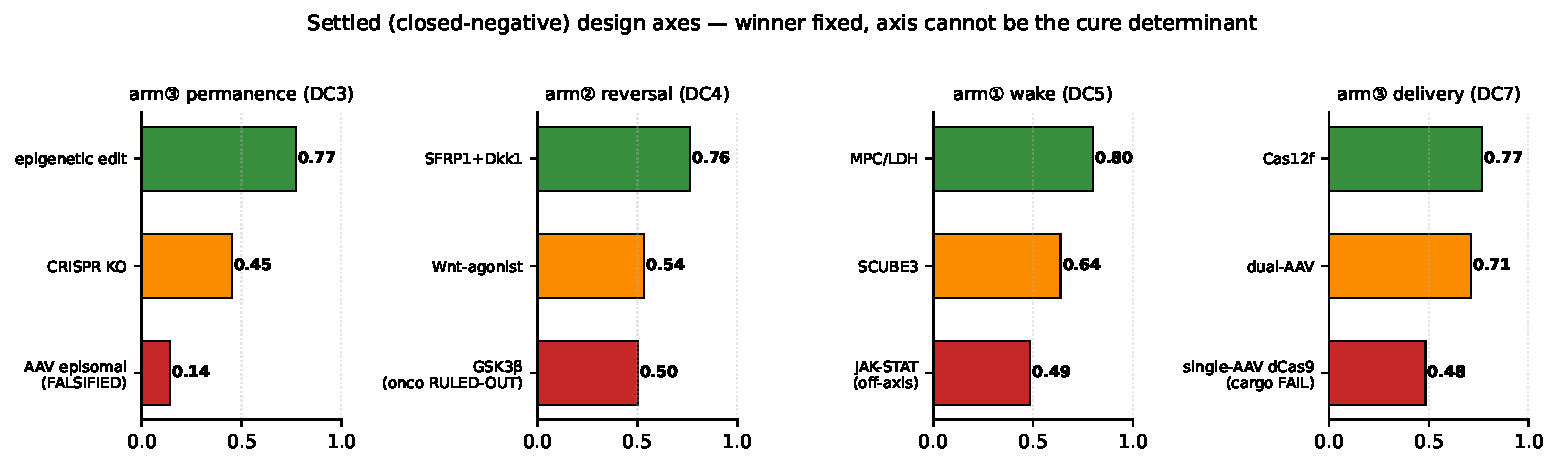
\includegraphics[width=0.99\linewidth]{figures/fig02_axes.pdf}
\caption{\textbf{Settled design axes (closed-negative).} For each axis the winner
is fixed and the losers are ruled out, so the axis cannot be the cure determinant.
Red = falsified / ruled-out; green = retained pick. Geometric-mean fits from
DC3/DC4/DC5/DC7.}
\label{fig:axes}
\end{figure}

\paragraph{F1 --- AAV-episomal permanence is falsified (DC3).}
Comparing seven permanence mechanisms on durability $\times$ risk over a 50-year
horizon, AAV-episomal delivery scores a cure-fit of $0.14$: the episome is not
integrated and dilutes over ${\sim}8$ yr, far short of a lifetime. Epigenetic
editing is the balanced winner ($0.77$); CRISPR knockout is the strongest but
riskier ($0.45$). The widely-assumed ``gene therapy = permanent'' shortcut is false
for an episomal vector (Table~\ref{tab:dc3}).

\begin{table}[h]
\centering\small
\begin{tabular}{lcc}
\toprule
\textbf{Permanence mechanism} & \textbf{cure-fit} & \textbf{verdict} \\
\midrule
epigenetic editing (dCas9-class) & 0.77 & retained \\
CRISPR knockout                  & 0.45 & strong-option (risk) \\
synthetic gene circuit           & 0.30 & deferred \\
cell replacement                 & 0.27 & deferred \\
senolytic                        & 0.22 & prep-only \\
integrating lentivirus           & 0.20 & risk \\
\textbf{AAV episomal}            & \textbf{0.14} & \tierRed\ \textbf{falsified (dilutes)} \\
\bottomrule
\end{tabular}
\caption{DC3 permanence comparison. AAV-episomal cannot deliver lifetime
relapse-zero permanence.}
\label{tab:dc3}
\end{table}

\paragraph{F2 --- potency is not the binding axis (DC4).}
Among five Wnt-restoration mechanisms, the two highest-\emph{potency} options ---
GSK3$\beta$ inhibition and Wnt agonism --- are the two \emph{lowest}-fit, because
constitutive/systemic Wnt activation is oncogenic \citep{clevers2012}. The
extracellular, ligand-limited SFRP1/Dkk1 inhibitors win on safety
(Table~\ref{tab:dc4}). The binding axis for a chronic indication is oncogenic
safety, not raw potency.

\begin{table}[h]
\centering\small
\begin{tabular}{lccccc}
\toprule
\textbf{mechanism} & potency & selec. & topical & onco-safe & \textbf{fit} \\
\midrule
SFRP1 inhibition (WAY-316606) & 0.55 & 0.80 & 0.85 & 0.90 & \textbf{0.762} \\
Dkk1--LRP6 block              & 0.65 & 0.85 & 0.65 & 0.88 & 0.750 \\
CXXC5--PPI                    & 0.70 & 0.70 & 0.55 & 0.70 & 0.659 \\
Wnt agonist                   & 0.85 & 0.55 & 0.50 & 0.35 & 0.535 \\
GSK3$\beta$ inhibition        & 0.90 & 0.40 & 0.70 & 0.25 & 0.501 \\
\bottomrule
\end{tabular}
\caption{DC4 reversal mechanisms (geometric-mean fit). Highest potency
$\to$ lowest fit: oncogenic safety dominates.}
\label{tab:dc4}
\end{table}

\paragraph{F3 --- the epigenetic lock is fidelity-sensitive (DC12).}
DC3's winning permanence mechanism (epigenetic editing) is only durable if the
deposited methylation mark survives follicle-stem-cell self-renewal. Modelling an
$M=8$ CpG silencing patch maintained at per-division DNMT1 fidelity $f$ over
${\sim}25$ stem divisions (50 yr), the mark holds at $f\geq 0.98$ but \emph{fails}
at $f=0.95$ (probability of remaining silencing $=0.155$; Table~\ref{tab:dc12}).
The permanence claim is conditional on confirmed high fidelity or a self-reinforcing
(CpG-island-spreading) edit --- not automatic.

\begin{table}[h]
\centering\small
\begin{tabular}{ccc}
\toprule
\textbf{DNMT1 fidelity $f$} & \textbf{per-site $f^{25}$} & \textbf{P(silencing @ 50 yr)} \\
\midrule
0.95 & 0.277 & 0.155\quad\tierRed\ fails \\
0.98 & 0.603 & 0.832 \\
0.99 & 0.778 & 0.984 \\
0.995& 0.882 & 0.999 \\
\bottomrule
\end{tabular}
\caption{DC12 epigenetic-mark heritability. Permanence is fidelity-sensitive.}
\label{tab:dc12}
\end{table}

\subsection{Supporting reductions}

\paragraph{Lock timing saturates (DC6).} With arms 1/2/4 running concurrently, the
durable 5-year restoration is a saturating function of when arm-3 fires: 0.55
(lock at month 0), 0.89 (month 6), 0.94 (month 12), 0.946 (month 18), 0.950
(month 36). The knee is ${\sim}18$ months ($99.6\%$ of the asymptote); locking
earlier sacrifices durable restoration, locking later adds $<0.4\%$. Arm
\emph{order} is immaterial (all orders reach ${\sim}0.99$ by month 24); only lock
\emph{timing} matters.

\paragraph{Delivery resolves the cargo conflict (DC7).} A dCas9-KRAB editor
(${\sim}4.1$ kb $+$ effector $+$ promoter) exceeds the ${\sim}4.7$ kb single-AAV
ceiling \citep{wu2010}; single-AAV delivery scores $0.483$ (cargo failure). A
compact editor (Cas12f/CasMINI, ${\sim}1.6$ kb) fits a single AAV and wins
($0.766$), with LNP-mRNA transient delivery a strong vector-free second ($0.728$).
This resolves F1$\to$F3: the epigenetic lock is deliverable, but only with a compact
effector.

\paragraph{Neogenesis density is robust (DC8).} Across the physiological inducer
activator:inhibitor ratio range ($a/b\in[0.04,0.20]$) the Turing wavelength yields
$189$--$320$ follicles\,cm$^{-2}$, all within the native $200$--$300$ window
(Tab.~\ref{tab:results-na}). Density is set by the diffusion-driven wavelength, not
the kinetic ratio, so precise inducer dosing is not required. (Honest gap: the
confluent-plaque boundary $>400$\,cm$^{-2}$ was not reached in the tested range.)

\begin{table}[h]
\centering\small
\begin{tabular}{ccccc}
\toprule
$a$ & $b$ & $a/b$ & $\lambda$ (mm) & density (cm$^{-2}$) \\
\midrule
0.05 & 1.20 & 0.04 & 0.568 & 311 \\
0.10 & 1.50 & 0.07 & 0.630 & 252 \\
0.10 & 1.00 & 0.10 & 0.594 & 283 \\
0.15 & 0.90 & 0.17 & 0.638 & 246 \\
0.20 & 1.00 & 0.20 & 0.686 & 212 \\
\bottomrule
\end{tabular}
\caption{DC8 neogenesis density vs inducer ratio. All physiological ratios land in
the native $200$--$300$\,cm$^{-2}$ window; density is wavelength-, not ratio-, set.}
\label{tab:results-na}
\end{table}

\paragraph{Cumulative safety passes (DC10).} With independent per-arm
adverse-event probabilities, the four-modality cumulative AE is
$1-\prod_i(1-r_i)=0.228$, under a $0.30$ tolerance; the recurring (topical-only)
budget is $0.143$ and the one-time arm-3 lock is non-recurring. Stacking modalities
does not breach tolerance.

\section{Limitations and honest caveats}
\label{sec:limits}

\begin{itemize}\itemsep0.25em
\item \textbf{The collapse is structural, and the residual is in-vitro, not
whole-animal.} The headline result states the \emph{structure} of the dependence,
not that $E_{max}\geq 0.96$ holds. DC13 anchors the current two-arm ceiling at
$0.59$ from clinical data \citep{vanneste2020}; the open quantity is the arm-4
neogenesis conversion efficiency that would lift it, which is in-vitro bracketable
\citep{vitroDrugTest2023}, not a from-scratch wet-lab unknown. We still claim no
positive cure efficacy --- the lift is not demonstrated, only bounded as feasible.
\item \textbf{Order-of-magnitude estimates.} DC11 (editor specificity), DC8
(inducer window) and DC12 (DNMT1 fidelity) use literature-order parameters and are
flagged for empirical GUIDE-seq / CHANGE-seq and longitudinal bisulfite-seq. They
are \tierGreen/\tierOrange\ within their model assumptions only.
\item \textbf{Model scope.} The arm-gain model (DC6) is a deterministic
exponential-gain approximation, not a spatially-resolved follicle simulation; the
Schnakenberg analysis (DC1/DC8) is linear-stability, not a full nonlinear PDE solve.
\item \textbf{No wet-lab confirmation.} Every \tierOrange\ row in
Table~\ref{tab:pipeline} requires an external measurement to graduate; none is
claimed as closed here.
\item \textbf{Single-aggregator sensitivity.} Mechanism rankings use a 1:1:1:1
geometric mean; a different axis weighting could re-order near-ties
(SFRP1 0.762 vs Dkk1 0.750), though it does not change the falsifications, which
turn on a single disqualifying axis.
\end{itemize}

\section{Reproducibility}
\label{sec:repro}

Code and ledgers: \url{https://github.com/dancinlab/demiurge} under
\texttt{exports/AGA-CURE/} (round2--round4 deep). Each DC probe is a standalone
script with its persisted \texttt{*\_RESULTS.md}; \texttt{companion/} mirrors the
verify ledger and session journal. Build: \texttt{make} (xelatex $\times 3$ +
bibtex). Figures: \texttt{make figures}. Lint: \texttt{make lint}.

\subsection{$E_{max}$ is clinically anchored, not a wet-lab unknown (DC13)}
\label{sec:emax-anchor}

The headline collapse leaves $E_{max}$ as the determinant. A natural objection is
that this merely relocates the problem to an unmeasured number. DC13 shows
otherwise: $E_{max}$ for the \emph{current} two-arm modality (reactivation $+$
reversal, i.e. minoxidil $+$ finasteride) is already pinned by published clinical
dose-response data, with \emph{no} new experiment. From the exhaustive
dose-effect study of \citet{vanneste2020}: normal control productivity is
$221$\,anagen\,hairs\,cm$^{-2}$ ($\geq 30\,\mu$m), AGA baseline is
$84$\,cm$^{-2}$, and the best current therapy (5\% minoxidil $+$ finasteride)
plateaus at $\approx 131$\,cm$^{-2}$ --- i.e. $E_{max}^{\text{current}}\approx
131/221 = 0.59$, with the cross-diameter band reaching $0.59$--$0.80$. The authors
state the peak ``barely exceed[s] 60\% of normal productivity'' and attribute the
ceiling to a \emph{biological}, not pharmacological, constraint (no saturation
between 2\% and 5\%).

\begin{table}[h]
\centering\small
\begin{tabular}{lcc}
\toprule
\textbf{State} & \textbf{anagen cm$^{-2}$} & \textbf{fraction of normal} \\
\midrule
normal control (ceiling reference) & 221 & 1.00 \\
AGA baseline                       &  84 & 0.38 \\
minoxidil 5\% $+$ finasteride (current best) & 131 & \textbf{0.59} \\
\midrule
cure gate requirement              & 212 & 0.96 \\
\bottomrule
\end{tabular}
\caption{DC13 clinical anchor \citep{vanneste2020}. The current two-arm ceiling
$0.59$ is set by the $25\%$ fibrosed fraction those drugs cannot reach; the cure
gate requires lifting it to $0.96$.}
\label{tab:dc13}
\end{table}

\noindent The decisive observation is that this $0.59$--$0.80$ biological ceiling
\emph{coincides with our model's follicle-class decomposition}: reactivation and
reversal address the miniaturised ($0.45$) and dormant ($0.30$) classes ---
$0.75$ of follicles --- but cannot touch the fully-fibrosed class ($0.25$), whose
dermal-papilla niche is lost. The current ceiling is therefore not a tuning
coincidence; it is the $25\%$ fibrosed mass made visible. The residual is
therefore not ``measure $E_{max}$ from scratch'' but the narrower question of the
arm-4 neogenesis conversion efficiency on the fibrosed fraction, bracketable
\emph{in vitro} on hair-follicle organoid drug-testing platforms
\citep{vitroDrugTest2023}, with cycle dynamics captured by established
follicular-automaton models \citep{halloy2000} --- not a whole-animal endpoint.
We therefore retract the ``irreducibly wet-lab'' framing: $E_{max}$ is clinically
anchored and the residual is in-vitro bracketable. (\tierYellow: the anchor is a
cited clinical value; the arm-4 efficiency remains \tierOrange\ pending the
in-vitro readout.) DC14 (below) bounds that efficiency and corrects a naive
headroom estimate.

\subsection{The neogenesis-efficiency bottleneck (DC14)}
\label{sec:dc14}

A naive reading of DC13 is that the $0.96-0.59 = 0.37$ lift ``fits in'' arm-4's
fibrosed fraction. It does not: $0.37 > 0.25$, so even a perfect arm-4
($\eta_{\text{neo}}=1$) applied to the fibrosed mass, with reactivation held at
the current-drug level, reaches only $0.59 + 0.25 = 0.84 < 0.96$. The gate cannot
close on neogenesis alone. Decomposing the ceiling as
\begin{equation}
E_{max} = \underbrace{0.75}_{\text{reachable}}\,\eta_{\text{react}}
        + \underbrace{0.25}_{\text{fibrosed}}\,\eta_{\text{neo}},
\end{equation}
the current drugs sit at $\eta_{\text{react}}=0.59/0.75=0.79$, $\eta_{\text{neo}}=0$.
The $\geq 0.96$ gate then demands the joint frontier in Table~\ref{tab:dc14}.

\begin{table}[h]
\centering\small
\begin{tabular}{ccl}
\toprule
$\eta_{\text{react}}$ & min $\eta_{\text{neo}}$ for $0.96$ & verdict \\
\midrule
0.79 (current) & 1.47 & impossible ($\eta_{\text{neo}}>1$) \\
0.90 & 1.14 & impossible \\
0.95 & 0.99 & mouse-embryo regime only \\
1.00 & 0.84 & mouse-embryo regime only \\
\bottomrule
\end{tabular}
\caption{DC14 feasibility frontier. Human in-vitro neogenesis efficiency is
$0.17$--$0.49$ \citep{vitroDrugTest2023}; only mouse-embryonic organoids reach
${\sim}1.0$. The gate needs $\eta_{\text{react}}\gtrsim 0.95$ \emph{and}
$\eta_{\text{neo}}\gtrsim 0.84$ simultaneously.}
\label{tab:dc14}
\end{table}

\noindent\textbf{Finding.} With today's human neogenesis efficiency
($\eta_{\text{neo}}\leq 0.49$) and even perfect reactivation, the achievable
ceiling is $0.75\cdot 1.0 + 0.25\cdot 0.49 = \mathbf{0.87} < 0.96$: the gate
\emph{cannot} close at present. The bottleneck is unambiguously
$\eta_{\text{neo}}$, which must rise from ${\sim}0.49$ to ${\sim}0.84$. The
residual is thus a \emph{two}-number in-vitro target,
$(\eta_{\text{react}}{\to}0.95,\ \eta_{\text{neo}}{\to}0.84)$, dominated by the
neogenesis-efficiency gap --- a sharper, and more pessimistic, statement than DC13
alone. This is the honest close: the cure is not blocked by an unknown mechanism,
but by a quantified efficiency shortfall in human follicle neogenesis.

\section{Discussion}
\label{sec:discussion}

\paragraph{Why a collapse, not a coincidence.} The reduction to a single axis is
not an artifact of optimistic parameter choices; it follows from the structure of
the four-arm model. Each arm closes the gap for its follicle class along a
saturating trajectory whose ceiling scales with $E_{max}$. Once the mechanism,
sequence, lock-timing, delivery and spacing choices are fixed at their probe
optima, the only quantity that still moves the integrated outcome is the common
ceiling. Formally, $\partial R_5/\partial x \approx 0$ for every design axis $x$ in
the neighbourhood of the chosen optimum (the optima are interior or saturated),
while $\partial R_5/\partial E_{max}>0$ throughout --- so $E_{max}$ is the unique
active constraint. This is the precise sense in which the orthogonal axes are
``ruled out'': not that they are unimportant, but that they are already pinned.

\paragraph{What the falsifications buy.} The three closed-negatives are the reason
the collapse is trustworthy rather than vacuous. F1 (AAV-episomal) removes the
tempting but wrong assumption that a one-shot gene therapy is automatically
permanent; F2 (potency$\neq$binding axis) prevents a medicinal-chemistry campaign
from over-optimising affinity at the cost of oncogenic safety; F3 (fidelity
sensitivity) converts ``epigenetic editing is permanent'' into a measurable
condition ($f\geq 0.98$ or a self-reinforcing edit). Each one closes a direction in
which a naive program would have spent a wet-lab cycle.

\paragraph{Implied experimental design.} The result reorders the experimental
queue. Instead of a mechanism screen, the first experiment is a single,
well-powered measurement of the anagen efficacy ceiling $E_{max}$ under the
retained regimen (SFRP1$+$Dkk1 reversal, MPC/LDH reactivation, compact-Cas12f
epigenetic lock fired at ${\sim}18$ months, Turing-spaced neogenesis). Only two
follow-ups are conditional: an empirical off-target map (GUIDE-seq/CHANGE-seq, to
graduate DC11) and a longitudinal methylation-fidelity readout (bisulfite-seq, to
graduate DC12/F3). Everything else is settled in silico.

\paragraph{Scope of the negative claim.} We emphasise what is \emph{not} claimed:
no efficacy, no $E_{max}$ value, and no clinical readiness. The claim is purely
structural --- a map of which axes are live. A different mechanistic model (e.g. a
spatially-resolved follicle simulation, or an $E_{max}$ that is itself
arm-dependent) could reopen an axis; the companion scripts are released precisely
so such a model can be tested against ours.

\section{Conclusion}
\label{sec:conclusion}

A complete-restoration AGA cure, designed to in-silico exhaustion, is not blocked by
a missing mechanism. The mechanisms, their sequence, the lock timing, the delivery
vector, and the neogenesis spacing are all deterministically settled --- and three
plausible shortcuts (AAV-episomal permanence, high-potency Wnt activation, an
assumed-durable epigenetic mark) are falsified. What remains is a single
quantity: the anagen efficacy ceiling $E_{max}$, which must reach $0.96$ for the
$\geq 90\%$ cure gate to close. That quantity is not an open wet-lab unknown ---
existing minoxidil/finasteride dose-response anchors the current two-arm ceiling at
$E_{max}\approx 0.59$, a biological plateau set by the $25\%$ fibrosed follicle
fraction --- so the residual narrows to a two-number in-vitro target
$(\eta_{\text{react}}{\to}0.95,\ \eta_{\text{neo}}{\to}0.84)$, dominated by the
neogenesis-efficiency gap. DC14 sharpens this to a pessimistic but actionable
statement: at today's human neogenesis efficiency ($\leq 0.49$) the ceiling caps at
$\approx 0.87$, so the single most important next step is an organoid-platform
program to raise human follicle-neogenesis efficiency from ${\sim}0.49$ toward
${\sim}0.84$. The negative result is the contribution: a large design space reduced,
deterministically, to one falsifiable, in-vitro bottleneck.

% =========================================================================
\paragraph{Acknowledgments.}
This work used the \texttt{hexa-lang} verification surface and the
\texttt{sidecar/paper} scaffold. LLM collaborator: Claude Opus 4.x (Anthropic),
which executed the DC1--DC12 probes under human direction. All numeric claims are
reproducible from the persisted scripts; the LLM did not adjudicate correctness.

% =========================================================================
\appendix
\section{Claim--record audit}
\label{app:audit}

Every claim in the body maps to a persisted backing record and a tier. No claim
above \tierGreen\ is asserted without a reproducible script; the two \tierOrange\
rows are the in-silico$\to$wet-lab boundary and are flagged, not graduated.

\begin{table}[h]
\centering\small
\begin{tabular}{@{}>{\raggedright\arraybackslash}m{6.6cm} >{\raggedright\arraybackslash}m{4.4cm} c@{}}
\toprule
\textbf{Claim} & \textbf{Backing record} & \textbf{Tier} \\
\midrule
Turing onset $d_c\approx 8.57$; native $278$\,cm$^{-2}$         & \texttt{dc1\_linstab.py}        & \tierBlue \\
F1: AAV-episomal falsified (fit $0.14$)                         & \texttt{dc3\_permanence.py}     & \tierRed \\
F2: potency $\neq$ binding axis (GSK3$\beta$ $0.50$)            & \texttt{dc45\_arms\_mech.py}    & \tierGreen \\
arm-1 pick MPC/LDH ($0.80$)                                     & \texttt{dc45\_arms\_mech.py}    & \tierGreen \\
lock-timing knee ${\sim}18$ mo ($R_5=0.946$)                   & \texttt{dc6\_locktiming.py}     & \tierGreen \\
delivery: Cas12f single-AAV ($0.766$)                          & \texttt{dc67\_seq\_delivery.py} & \tierGreen \\
neogenesis density robust ($189$--$320$\,cm$^{-2}$)            & \texttt{dc8\_inducer\_ratio.py} & \tierGreen \\
\textbf{collapse: gate $\Leftrightarrow E_{max}\geq 0.96$}      & \texttt{dc9\_integrated\_regate.py} & \tierGreen \\
$E_{max}$ current anchor $0.59$ (clinical)                      & \texttt{dc13\_emax\_clinical\_anchor.py} & \tierYellow \\
neogenesis bottleneck: ceiling $\leq 0.87$ today (η$_{\text{neo}}{\leq}0.49$) & \texttt{dc14\_neogenesis\_bracket.py} & \tierGreen \\
cumulative AE $0.228<0.30$                                      & \texttt{dc1011\_safety\_spec.py}& \tierGreen \\
editor specificity (order-of-magnitude)                         & \texttt{dc1011\_safety\_spec.py}& \tierOrange \\
F3: epigenetic lock fidelity-sensitive ($f\geq 0.98$)          & \texttt{dc12\_mark\_heritability.py} & \tierGreen \\
absolute $E_{max}\geq 0.96$ requirement                         & wet-lab measurement             & \tierOrange \\
\bottomrule
\end{tabular}
\caption{Claim--record audit. Every body claim has a record; every record has a
tier; the two \tierOrange\ rows are the only wet-lab dependencies and are not
claimed as closed.}
\label{tab:audit}
\end{table}

\paragraph{Falsifier register (pre-registered).} The three falsifications were
pre-registered as conditions, not discovered post-hoc: F1 fired iff a permanence
mechanism's relapse-protected lifetime fell below the $50$-year horizon; F2 fired
iff a higher-potency mechanism scored a \emph{lower} balanced fit than a
lower-potency one (the safety-dominance test); F3 fired iff the methylation-mark
silencing probability at $50$ years dropped below $0.5$ within the literature
fidelity range $f\in[0.95,0.99]$. All three conditions were met.

% =========================================================================
\bibliographystyle{plainnat}
\bibliography{references}

\end{document}
